\section{Results}
\label{sec:results}

%\emph{Benchmarks (test results) and possibly competition results.  Include explanations and analyses of your results. As mentioned under “Benchmarks and comparisons” below, it is usually a clear strength if you have some results to com- pare, e.g. two different versions of your client with different methods/features/parameters.  You could also compare the behaviour of your client on different individual levels that illustrate a certain point, e.g. similar levels resulting in large differences in the client’s behaviour.}

To showcase how efficient our goal prioritisation technique is and how we have improved upon it throughout the project, we present some test runs using the \texttt{SAOptimal} level.
In the following we will refer to our main goal prioritisation technique (\cref{methods:goal_ordering}) as the ``complex'' prioritisation, and the ``simple'' differs in that it does not perform the final matrix computation as presented in \cref{methods:goal_ordering}.
The intuition is that goals placed in dead-ends or corners must be achieved before any goals that would otherwise block the path to the inner most goals.

We illustrate two different runs; one with simple goal prioritisation (\cref{fig:simple priority}) and one without goal prioritisation (\cref{fig:no priority}).

% Example of cells 
\begin{figure}[h!]
  \centering
  \begin{minipage}{.45\columnwidth}
    \centering
    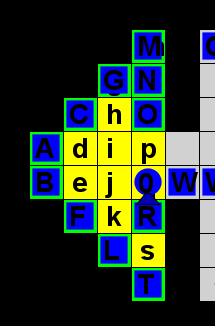
\includegraphics[height=5cm]{graphics/simple_priority_block.PNG}
    \caption{\label{fig:simple priority}Simple goal prioritisation.}
  \end{minipage}%
  \hspace{20pt}%
  \begin{minipage}{.45\columnwidth}
    \centering
    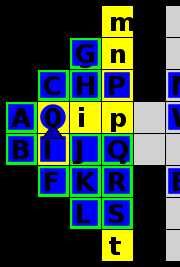
\includegraphics[height=5cm]{graphics/no_priority_block.png}
    \caption{\label{fig:no priority}No goal prioritisation.}
  \end{minipage}
\end{figure}

The main difference between the complex and simple prioritisation is that the complex forces and order on grouped goals.
The lack of strict order in apparent in the example of the simple prioritisation as illustrated in \cref{fig:simple priority}.
The agent chooses to place \textbf{R} before \textbf{S} and thus blocking the path to that goal.
Both goals have the same priority, but the complex goal prioritisation manages to solve this level with 31 fewer moves than the simple prioritisation as presented in \cref{tab:SAOptimal_results}.

\begin{table}[h!]
  \centering
  \begin{tabular}{@{}ll@{}}
    \toprule
    Prioritisation technique & Actions \\ 
    \midrule
    None    & $>1400$ \\ 
    Simple  & $761$ \\ 
    Complex & $730$ \\
    \bottomrule
  \end{tabular}
  \caption{\label{tab:SAOptimal_results}No. actions performed on \texttt{SAOptimal} level with different prioritisation techniques.}
\end{table}

Furthermore, we also ran the level without any particular prioritisation technique to choose which goal to achieve first.
For this reason the goals are fulfilled in an arbitrary order, which yields a solution that require almost more than double the actions than with some prioritisation.
Many unnecessary moves are wasted because the inner most goals are left open.

\subsection{Performance vs. Optimality}
\label{sec:performance vs. optimality}

We have developed a client with performance in mind.
The only technique we used to give better results was to develop the goal prioritisation technique, so the client did not fill in goals arbitrarily.
For course's competition presentation we found that, as an example, our client was beaten in \texttt{SAOptimal} with 7 \% less actions performed. 
However, our client solved the level approximately 700 times faster than the opponent.

Note that we performed our tests on a laptop with Intel® Core™ i5 4210U Processor 2.7 GHz, 4GB DDR3L 1600 MHz SDRAM, with an SSD hard drive.
